\chapter{Grundlagen}
\label{cha:Grundlagen}
Im folgenden Kapitel werden die Grundlagen vorgestellt, auf denen die Modellierung der Wasserstoffkomponenten aufbaut.\\
Im ersten Abschnitt wird dazu auf die Eigenschaften verschiedener Modellstrukturen eingegangen. Weiterhin wird ein Überblick über den aktuelle Stand der Modellierung von Elektrolyseuren und Brennstoffzellen geliefert.\\
Im zweiten Abschnitt wird die Funktionsweise von Elektrolyseuren und Brennstoffzellen erläutert. Darauf aufbauend wird auf die zur Modellierung genutzten physikalischen Grundlagen eingegangen.\\ 

\section{Modellierung von Elektrolyseuren und Brennstoffzellen}
Nach \citet[S.~32]{tabeling_softwaresysteme_2006} ist ein Systemmodell eine Abstraktion zu einem System (im Sinne des Systemgebildes) welche nur eine Menge ausgewählter, gerade interessierender Sachverhalte des betrachteten Systems aufweist. Das Ziel der Modellierung ist daher nicht alle Eigenschaften des realen Systems möglichst exakt wiederzugeben sondern ausgewählte Eigenschaften ausreichend genau zu beschreiben.\\

\begin{figure}[h]
	\centering
		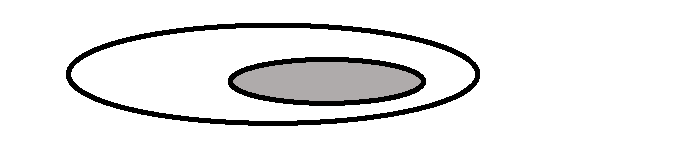
\includegraphics[scale=1]{Figures/Modell-System.pdf}
		\caption{Überdeckung der Eigenschaften von System und Modell nach \citet{tabeling_softwaresysteme_2006}.}
\label{fig:Modell-System}	
\end{figure}

Nach \citet{sjoberg_nonlinear_1995} liegt die Schwierigkeit in der Modellierung in erster Linie in der Identifikation einer zur Anwendung geeigneten Modell Struktur. Üblicherweise werden dabei drei Gruppen unterschieden: White-, Grey- und Black-Box-Modelle. White-Box-Modelle erfordern ein umfassendes Verständnis des realen Systems und bauen vollständig auf physikalischem Vorwissen auf. Ziel ist eine exakte, auf physikalischen Gesetzen basierende Modellierung. Black-Box-Modelle hingegen nutzten kein Vorwissen, sondern verwenden aus Experimenten gewonnene Daten. Dabei schätzen sie das Systemverhalten als eine Kombination mehrerer Eingangs- und dazu gehöriger Ausgangsgrößen ab \citep{hauth_grey-box_2008}. Häufig liegen verwendete Modelle zwischen den beiden genannten Fällen, es handelt sich also meist um Grey-Box-Modelle. Dies lassen sich wiederum in zwei Untergruppen unterteilen: Bei physikalischen Grey-Box-Modellen wird physikalisches Vorwissen genutzt und mit experimentell gewonnenen Parametern ergänzt. Bei semiphysikalischen Grey-Box-Modellen wird Vorwissen über das Systemverhalten genutzt, um eine Modellstruktur für ein Modell mit Black-Box Charakter zu entwickeln.\\
\citet{sjoberg_nonlinear_1995} geben als Basisregel an, dass vorhandenes Wissen über das Systemverhalten bei der Modellierung genutzt werden sollte. Dies lässt sich darin begründen, dass experimentell gewonnene Datensätze nur Teilbereiche eines komplexen Systems beschreiben können und daher in ihrer Allgemeingültigkeit eingeschränkt sind. Als Nachteil der physikalischen Modellierung ist zu benennen, dass mit steigender Systemkomplexität die Entwicklungs- und Rechenzeit erheblich zunimmt \citep{hauth_grey-box_2008}. In Tabelle \ref{tb:Modellstrukturen} sind grundlegende Eigenschaften von White- und Black-Box-Modellen zusammengefasst. \\

\begin{table}[ht]
		\centering
		\caption{Eigenschaften verschiedener Modellstrukturen.}
		
\begin{tabular}{l l}
		\toprule
		White-Box-Modell & hohes Maß an implementierter Systemkenntnis\\
		& $+$ großer Gültigkeitsbereich\\
		& $-$ lange Rechendauer und Entwicklungsdauer bei komplexen Systemen\\
		\midrule
		Black-Box-Modell & große Menge an Eingangsdaten\\
		& $+$ geringer Entwicklungs- und Rechenaufwand bei komplexen Systemen\\
		& $-$ eingeschränkter Gültigkeitsbereich\\
		\bottomrule
		\end{tabular}
		\label{tb:Modellstrukturen}
		\end{table}	

\subsection{Stand der Technik der Modellierung von Elektrolyseuren}
Im Folgenden wird ein kurzer Überblick über Aktuelle Forschungsergebnisse zur Modellierung von Elektrolyseuren geliefert:\\

\citet{ulleberg_modeling_2003} präsentiert ein semi-physikalisches Modell einer alkalischen Elektrolyse-Zelle zur Bestimmung der Polarisationskurve. Dabei wurden als Einflussparameter die Betriebstemperatur und der Druck berücksichtigt. Der Zusammenhang von elektrischer Leistung und produzierter Stoffmenge wird durch eine Kombination aus physikalischen Gesetzen und aus Messwerten gefolgerten Approximationen bestimmt. \citet{amores_influence_2014} ergänzen dieses Modell um weitere Einflussparameter um den Gültigkeitsbereich des Modells zu vergrößern. Die Parameter wurden dabei mithilfe eines Matlab Fitting-Codes aus experimentell gewonnenen Messwerten bestimmt.\\

\citet{tjarks_pem-elektrolyse-systeme_2017} stellt ein physikalisches Modell eines PEM-Elektrolyseurs für die Untersuchung von Power-to-Gas Anwendungen vor. Dabei werden physikalische Gesetze verwendet, um Verlustmechanismen zu beschreiben. Weiterhin wird das Zellverhalten mit Fitting Parametern den Messwerten einer Versuchsreihe angenähert. Eine Besonderheit des Modells ist die Berücksichtigung des Thermomanagements des Elektrolyseurs zur Berechnung der benötigten Heiz- beziehungsweise Kühlleistung. Zudem werden zum Betrieb des Elektrolyseurs benötigte Systemkomponenten in der Modellierung berücksichtigt.\\

\citet{rodriguez_cfd_2020} modellieren neben den elektrochemischen Vorgängen in einem Elektrolyseur auch die Strömungsvorgänge, die den Stofftransport beschreibenden. Dabei werden die Vorgänge der Blasenbildung und Strömung von Gasen mithilfe einer CFD-Simulation berücksichtigt. Die Abweichungen der Simulationsergebnisse von Messwerten einer Einzelzelle liegt unter 1\%, wobei zu bedenken ist, dass die Methode eine genaue Kenntnis der Zellgeometrie, der Eigenschaften der verwendeten Materialien und weiterer Parameter erfordert.\\

Nach aktuellem Stand wird somit eine Anzahl verschiedener Modellierungsansätze genutzt, um das Verhalten von Elektrolysezellen vorherzusagen. Häufig werden physikalische Modelle verwendet, da diese einen Mittelweg zwischen der benötigten Datenmenge und dem Entwicklungsaufwand darstellen. Der Detaillierungsgrad variiert dabei abhängig vom Untersuchungsfokus. Nachteile aktueller Modelle sind die Beschränkung auf eine Elektrolyse-Technologie.

\subsection{Stand der Technik der Modellierung von Brennstoffzellen}
Brennstoffzellen weisen hinsichtlich der Modellierung große Ähnlichkeiten zu Elektrolysezellen auf. Beispielsweise implementieren \citet{motapon_development_2012} oder \citet{chugh_experimental_2020} die gleichen physikalischen Gesetzt in einem Modelle für Brennstoffzellen die  von \citet{tjarks_pem-elektrolyse-systeme_2017} in dem Elektrolyseur-Modell implementiert sind.

\citet{barragan_iterative_2020} präsentieren ein Black-Box Modell zur Echtzeitregelung von Brennstoffzellen.
Das Modell basiert auf der Fuzzy Methode, welche aus Paaren von Eingangs- und Ausgangsdaten Merkmale ableitet.
Abhängig davon, in welchem Maß die Eingangswerte die Merkmale erfüllen, werden Ausgangsdaten der Versuchsreihen überlagert, um die Ausgangswerte abzuschätzen. 
Kombiniert wird die Fuzzy Methode mit einem Kalman Filter. 
Dieser rekursive Filter, schätzt das Datenrauschen auf Grundlage von Messwerten ab und ermöglicht es, die Ausgabe iterativ zu bestimmen. 
Das Modell ist besonders vorteilhaft für die Langzeit-Regelung von Brennstoffzellen, weil laufend Input-Output Daten in die Modellierung einfließen.\\

\citet{jiao_challenges_2017} untersuchen den aktuellen Stand der physikalischen PEM-Brennstoffzellen Modellierung und arbeitet Schwächen der aktuellen Modellierungsansätze aus. Das Wassermanagement der Zelle wird als wichtiges Forschungsfeld angeführt, da die Membran zur höheren Leitfähigkeit ausreichend befeuchtet sein muss.
Es werden numerische Modelle vorgestellt, die entwickelt wurden, um Verdampfungsvorgänge sowie die Mehr-Phasen-Strömung in den Kanalstrukturen zu beschreiben. Als Nachteil stellt sich dabei die hohe benötigte Rechenleistung heraus.
Weiterhin bleibt die Eisbildung, welche besonders im Falle eines Kaltstarts auftritt und die Katalysator-Flächen bedecken kann, in den Verfahren unberücksichtigt.\\

Wie auch bei der Modellierung von Elektrolysezellen, existieren somit nach aktuellem Stand eine Anzahl verschiedener Modellierungsansätz für Brennstoffzellen. Meist beschränken sich die Modelle auf die Modellierung der elektrischen Ausgangsleistung zur Nutzung in für mobilen Anwendungen. Ein weiterer Nachteile aktueller Modelle ist die Beachtung von nur einer Elektrolyse-Technologie.

\section{Grundlagen der Wasserelektrolyse}
\label{sec:Elektrolyse}
Im folgenden Abschnitt werden anfangs die elektrochemischen Grundlagen der Elektrolyse von Wasser vorgestellt sowie deren thermodynamische Zusammenhänge geschildert.
Zudem wird die ideale Zellspannung hergeleitet und wesentliche Verlustmechanismen sowie deren Einfluss auf den Betriebsbereich von Elektrolyseuren beschrieben.
Weiterhin werden drei technische Lösungen der Wasserelektrolyse vorgestellt, sowie Gemeinsamkeiten und Unterschiede von Elektrolyseuren und Brennstoffzellen aufgezeigt.
Abschließend wird auf Komponenten eingegangen, die zum Betrieb von Elektrolyseuren und Brennstoffzellen benötigt werden.\\

Als Elektrolyse bezeichnet man einen chemischen Prozess, bei dem eine Redoxreaktion durch elektrische Spannung erzwungen wird. 
Um eine kontrollierbare Durchführung der Reaktion sicherzustellen, ist eine räumliche und elektrische Trennung der Oxidation und Reduktion nötig \citep{tjarks_pem-elektrolyse-systeme_2017}. Allerdings muss der Ionenaustausch zwischen Anode und Kathode möglich sein und dies wird durch ein Elektrolyt erreicht.\\

Bei der Wasserelektrolyse wird dieses Prinzip angewendet, um aus Wassermolekülen elementaren Wasserstoff und Sauerstoff zu gewinnen. Dabei liegt die folgende allgemeine Reaktionsgleichung vor:   
\begin{align}
	\label{gl:Reaktionsgleichung}
	\ce{H2O &-> H2 + 1/2O2}
\end{align}
Die allgemeine Reaktionsgleichung ist dabei unabhängig vom Elektrolyt, wohingegen sich die Oxidations- und Reduktions Gleichungen unterscheiden. Die Oxidation findet an der Anode statt und hat Sauerstoff als Produkt. An der Kathode wird durch die Reduktion Wasserstoff gebildet. Es gibt drei mögliche Ladungsträger bei der Wasserelektrolyse, welche in Abbildung \ref{fig:LadungstraegerBeiDerWasserelektrolyse} gezeigt werden: Hydroxidionen, Protonen oder Oxidionen \citep{tjarks_pem-elektrolyse-systeme_2017}. Zu den verschiedenen Ladungsträgern werden im Unterkapitel  \ref{subsec:Technologien der Wasserelektrolyse} technische Verfahren erläutert.\\

\begin{figure}[h]
	\centering
		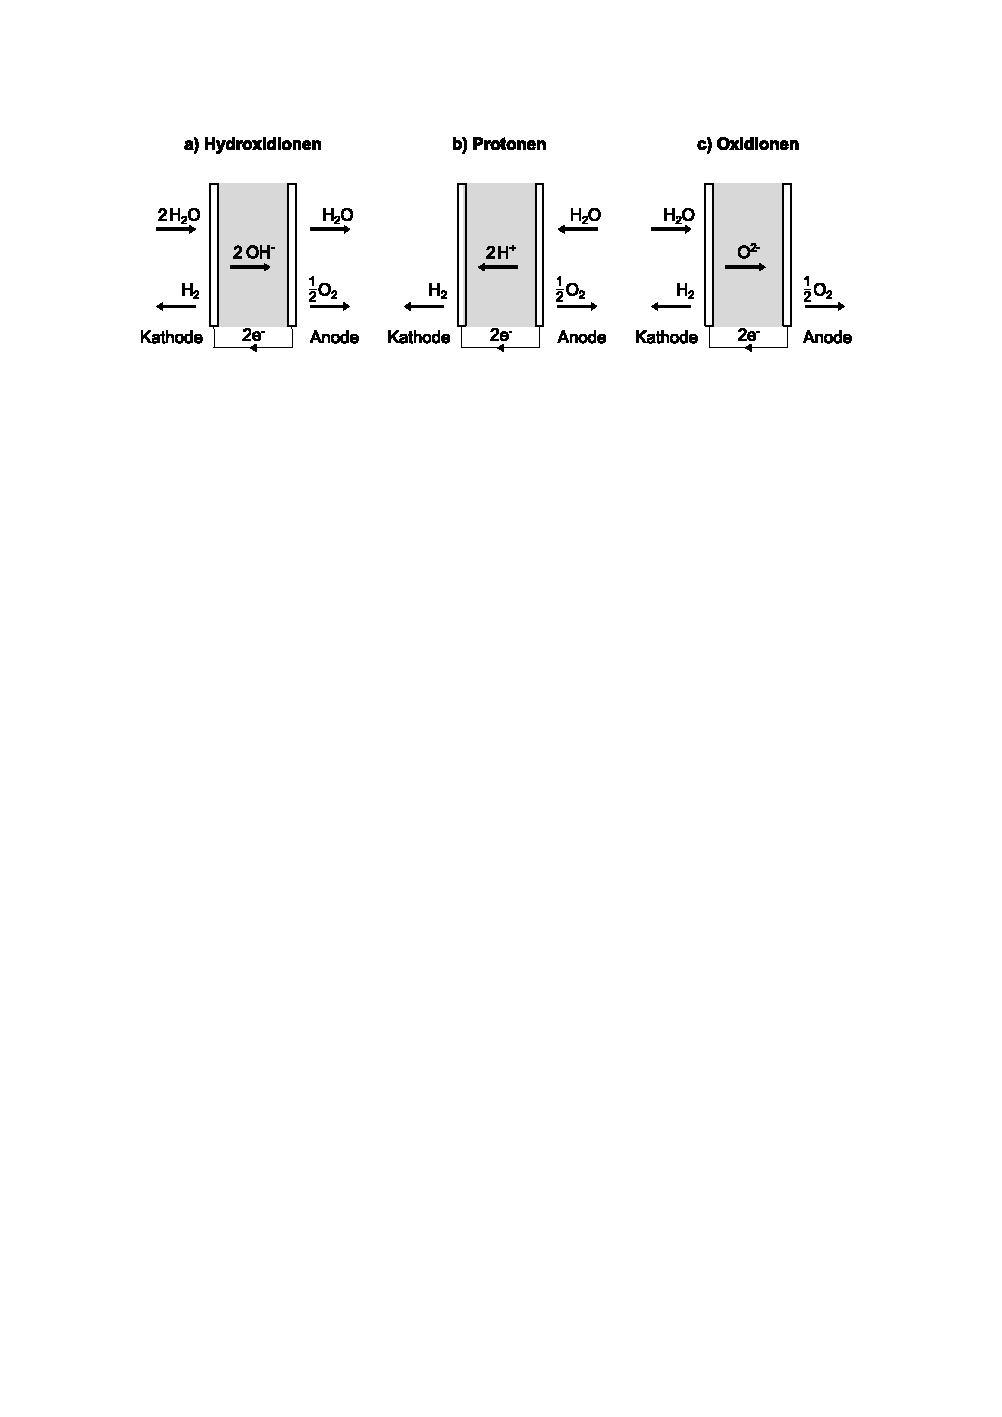
\includegraphics[scale=1]{Figures/LadungstraegerBeiDerWasserelektrolyse}
		\caption{Ladungsträger bei der 
		Wasserelektrolyse nach \citet{tjarks_pem-elektrolyse-systeme_2017}.}
\label{fig:LadungstraegerBeiDerWasserelektrolyse}	
\end{figure}

\subsection{Elektrochemische Betrachtung}
\label{subsec:Elektrochemische Betrachtung}
Die benötigte Energie bei einer Redoxreaktion entspricht der Reaktionsenthalpie $\Delta_R H$ und lässt sich aus den Bildungsenthalpien ($\Delta_f H_i$) und stöchiometrischen Koeffizienten ($\nu_i$) der Edukte und Produkte bestimmen \citep{falcao_review_2020,brauns_alkaline_2020}:
\begin{align}
 	\Delta_R H = \sum{\nu_i \cdot \Delta_f H_i}
\end{align}
Unter der Annahme, dass die nötige thermische Energie vorliegt, entspricht die zur Reaktion benötigte elektrische Energie  der freien Reaktionsenthalpie $\Delta_R G$, welche sich über die Reaktionsentropie $\Delta_R S$ errechnen lässt \citep{falcao_review_2020,brauns_alkaline_2020}.
\begin{align}
	\Delta_R G = \Delta_R H - T \cdot \Delta_R S \\
 	\Delta _R S = \sum{\nu_i S_i}
\end{align}

Für die Wasserelektrolyse (\ref{gl:Reaktionsgleichung}) bei Standardbedingungen ($T_0 = \SI{25}{\degreeCelsius}$ und $p_0 = \SI{101,325}{\kilo\pascal}$) ergibt sich mit den Daten aus Tabelle \ref{tb:Stoffdaten} die Reaktionsenthalpie zu $\Delta H^0_R = \SI{285,25}{\kilo\J\per\mol}$ und die freie Enthalpie zu $\Delta G^0_R = \SI{236,59}{\kilo\J\per\mol}$. Es liegt dabei eine starke Temperaturabhängigkeit vor, was in Abbildung \ref{fig:Entropien} deutlich wird.

\begin{table}[ht]
		\centering
		\caption{Standardbildungsenthalpien und Standardentropien für $\SI{25}{\degreeCelsius}$ \citep{koj_entwicklung_2021} sowie stöchiometrische Koeffizienten aus Gleichung \ref{gl:Reaktionsgleichung}.}
		
\begin{tabular}{c c c c}
		\toprule
		\multirow{2}{*}{Komponenten i} & 
		\multicolumn{1}{c}{$\Delta_f H^0_i$} & 
		
		\multicolumn{1}{c}{$S^0_i$} &
		
		\multicolumn{1}{c}{$\nu_i$}
		\\
		& 
		\multicolumn{1}{c}{$\textrm{[kJ/mol]}$}& 
		
		\multicolumn{1}{c}{$\textrm{[J/(molK)]}$} &
		\multicolumn{1}{c}{$\textrm{[---]}$}
		\\
		\midrule
		$\ce{H2O}$ & -285,25 & -216.35 &  -1\\
		$\ce{O2}$ & 0 &  21,78 &  $\textrm{1/2}$\\
		$\ce{H2}$ & 0 &  19,88 &  1\\
		\bottomrule
		\end{tabular}
		\label{tb:Stoffdaten}
		\end{table}	
			
\paragraph{Reversible Zellspannung}
\label{par:rev Zellspannung}
Mit der Faraday Konstante ($F=\SI{96485,3}{\coulomb\per\mol}$) und der Anzahl der pro Reaktion transferierten Elektronen ($z = 2$) lässt sich die thermoneutrale Spannung bei Standardbedingungen $U^0_{tn}$ sowie die reversible Zellspannung bei Standardbedingungen $U^0_{rev}$ errechnen \citep{falcao_review_2020}. 

\begin{align}
 U^0_{tn} = \frac{\Delta H^0_R}{zF} = \SI{1,478}{\volt}\\
 U^0_{rev} = \frac{\Delta G^0_R}{zF} = \SI{1,226}{\volt}
\end{align}

Der im vorherigen Abschnitt erläuterte Temperatureinfluss auf die Reaktionsbedingungen wirkt sich auch auf die reversible und thermoneutrale Spannungen aus (Abbildung \ref{fig:Entropien}). Häufig wird dieser Zusammenhang durch Gleichung \ref{gl:dT} abgebildet \citep{olivier_low-temperature_2017}.
Weiterhin liegt für die Zellspannung eine Abhängigkeit von den Produkt- und Edukt Aktivitäten vor, welche durch die Nernst Gleichung beschrieben werden kann. Drückt man die Aktivität der Produktgase über das Verhältnis des Partialdrucks zum Standarddruck $p_0$ aus, ergibt sich der in Gleichung \ref{gl:dp} angeführte Zusammenhang.\\

\begin{align}
U_{rev} = U^0_{rev} + \Delta U_{rev}(p) + \Delta U_{rev}(T)
\label{gl:Urev}\\
\Delta U_{rev}(T) = - 8,5 \cdot 10^{-4} \cdot (T-298)
\label{gl:dT}\\ 
\Delta U_{rev}(p) = \frac{RT}{zF}\ln{ \Bigl( \frac{p_{H_2}/p_0 \sqrt{p_{O_2}/p_0}}{a_{H_{2}O}}  \Bigr) } 	
\label{gl:dp}
\end{align} 

\begin{figure}[h]
	\centering
		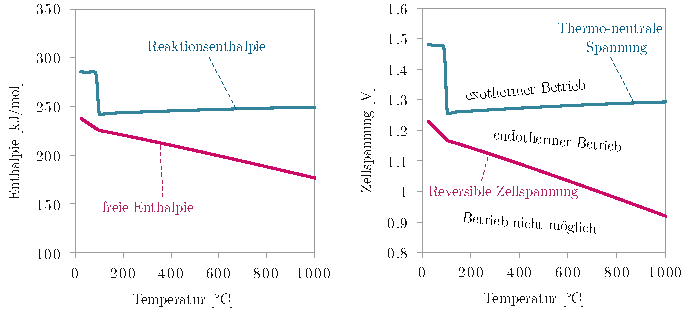
\includegraphics[scale=1]{Figures/VerlaufVonEntropien}
		\caption{Abhängigkeit der Reaktionsenthalpie und der freien Enthalpie von der Temperatur nach \citet{tremel_electrolysisfundamental_2018}.}
\label{fig:Entropien}	
\end{figure}

\subsubsection{Überspannungen}
\label{subsubsec:Überspannungen}
Die reale Zellspannung $U_{real}$ ist im Betrieb aufgrund von Verlusten immer größer als die reversiblen Zellspannung. Ist die reale Zellspannung niedriger, als die thermoneutrale Spannung, läuft das System endotherm ab. In dem Fall muss dem System Wärmeenergie zugeführt werden.\\
Als maßgeblichen Verluste, auch Überspannungen genannt, werden üblicherweise drei Phänomene betrachtet: Aktivierungsverluste ($U_{Akt}$), Ohmsche Verluste ($U_{Ohm}$) und Konzentrationsüberspannung \citep{falcao_review_2020}. In dieser Arbeit werden die Konzentrationsüberspannungen als vernachlässigbar klein angenommen, da sie erst außerhalb der üblichen Betriebsgrenzen von signifikanter Größenordnung sind. Ein weiteres Phänomen sind Diffusionsströme von Wasserstoff auf die Anodenseite und von Sauerstoff auf die Kathodenseite, allerdings sind diese aus Sicherheitsaspekten gering zu halten, was in \ref{subsec:Polarisationskurve} näher erläutert wird. Daher werden Diffusionsströme in dieser Arbeit vernachlässigt. Somit wird die reale Zellspannung wie folgt berechnet:\\

\begin{align}
	\label{gl:U_realEL}
	U_{real} =  U_{rev} + U_{Akt} + U_{Ohm}
\end{align}   

\paragraph{Aktivierungsverluste} kommen durch die elektrochemischen Vorgänge an den Oberflächen er Elektroden und ihrer Kinetik zustande. Dabei treten zwei Phänomene auf:  Einerseits chemische (wegen des chemischen Gleichgewichtszustands der Ionen an der Grenzfläche zwischen Elektrode und Elektrolyt) und andererseits elektrische (aufgrund des Ladungstransports durch das elektrische Feld an der Grenzfläche) \citep{stempien_solid_2013}. Aktivierungsverluste lassen sich mithilfe der Butler-Volmer-Gleichung beschreiben \citep{olivier_low-temperature_2017,stempien_solid_2013}. Zur Modellierung kann für ausreichend hohe Stromdichten vereinfachend die Tafel- Gleichung angewendet werden, \citet{abdin_modelling_2015} nutzen sie in der folgenden Form:\\

\begin{align}
	U_{Akt} = \frac{RT}{ 2 \cdot \alpha
		\cdot F} \cdot ln(i/i_0)
\label{gl:Akt}
\end{align}

Der Durchtrittsfaktor $\alpha$ und die Austauschstromdichte $i_0$ sind dabei experimentell zu ermitteln und unterscheiden sich je nach Bauart.\\

\paragraph{Ohmsche Verluste} werden durch elektrische sowie ionische Widerstände und Kontaktwiderständen zwischen den Komponenten verursacht. Ionischen Widerstände, welche sich in dem Elektrolyt  und an den Elektrodenoberflächen lokalisieren lassen, dominieren üblicherweise die Ohmschen Verluste \citep{stempien_solid_2013,milewski_modeling_2014}. Elektrisch Widerstände treten in den Elektroden und an den Kontakten der Zelle auf und lassen sich somit durch einen günstigen Aufbau der Zelle vermindern \citep{tjarks_pem-elektrolyse-systeme_2017}. Die ohmschen Verluste können mithilfe des Ohmschen-Gesetztes (Gleichung \ref{gl:Ohm}) bestimmt werden, für welches neben dem Elektrodenabstand auch die Leitfähigkeit des Elektrolyts benötigt wird.\\ 
\citet{olivier_low-temperature_2017} geben eine Gleichung zur Berechnung der Leitfähigkeit alkalischer Zellen an, dabei sind die Einflussfaktoren die Betriebstemperatur ($T$) sowie die Stoffmengenkonzentration ($m$) der Lauge des Elektrolyts. Die Berechnung der Leitfähigkeit für Festoxid (SO) Zellen ist \citet{hajimolana_mathematical_2011} entnommen. 
Der Ansatz für PEM-Zellen wird in der Literatur häufig verwendet \citep{falcao_review_2020, olivier_low-temperature_2017} und beachtet neben der Betriebstemperatur ($T$) auch den Feuchtegehalt der Membran ($\lambda$). \citet{tjarks_pem-elektrolyse-systeme_2017}  erweitert die Berechnung des ohmschen Wiederstandes nach Gleichung \ref{gl:Ohm2} um einen Parameter zur Berücksichtigung elektrische Widerstände $R_{el}$.

\begin{align}
	U_{Ohm} = &i \cdot (\delta / \sigma)
\label{gl:Ohm}\\
	U_{Ohm,PEM} = &  i \cdot (\delta / \sigma + R_{el})
\label{gl:Ohm2}
\end{align} \begin{align}
	\sigma _{Alk} = &   -2.04m -0.0028m^2  + 0.005332mT  \notag\\
				&+207.2m/T +0.001043m^3-3 \cdot 10^{-3}m^2T^2\\[2pt]
	\sigma _{SO} = &  3.34 \cdot 10^4 + exp(-10300/T)\\
	\sigma _{PEM} = &  (0.005139 \cdot \lambda -0.00326) \cdot \exp(1268 \cdot (1/303-1/T))
\end{align}

\subsection{Thermisches Verhalten}
\label{subsec:Thermisches Verhalten}
Zur Bestimmung des Wärmeflusses wird nach \citet{webster_implementation_2019} die Energiebilanz einer Elektrolysezelle betrachtet: 

\begin{align}
	C_{Zelle} \frac{\mathrm{d}T}{\mathrm{d}t} = \dot{n} (h_{ein} - h_{aus}) + P_{el} - \dot{Q} 
\end{align} 

Die Enthalpiedifferenz ergibt sich aus der Reaktionsenthalpie und der Temperaturdifferenz zwischen Eingang und Ausgang. Die benötigte Reaktionsenthalpie und die elektrische Leistung drückt \citet{webster_implementation_2019}	über die Thermoneutrale Spannung und die Zellspannung aus. Unter der Annahme, dass die   Ausgangstemperatur der Gase gleich der Betriebstemperatur ist, ergibt sich für die Energiebilanz damit:  
 
\begin{align}
	C_{Zelle} \frac{\mathrm{d}T}{\mathrm{d}t} = &-(\dot{n}_{H2, ein} \cdot c_{p, H2} +\dot{n}_{H2, ein} \cdot c_{p, O2}) \cdot (T_{ein} - T) \notag\\
	 &- I \cdot (U_{Zell} - U_{tn}) - \dot{Q}
	\label{gl:Energiebilanz}
\end{align}

\subsection{Polarisationskurve und Betriebsbereiche von Elektrolyseuren}
\label{subsec:Polarisationskurve}
Die Polarisationskurve gibt die Abhängigkeit der realen Zellspannung $U_{real}$ eines Elektrolyseurs von der Stromdichte graphisch wieder.  Diese wird von vielen Faktoren, wie beispielsweise den Elektrodenmaterialien, der Geometrie der einzelnen Bauteile oder den Betriebsbedingungen wie Druck und Temperatur, beeinflusst. Grundlage für die Berechnung der Polarisationskurve ist die in \ref{par:rev Zellspannung} hergeleitete reversible Zellspannung und Gleichung \ref{gl:U_realEL}. In Abbildung \ref{fig:PolarisationskurveElektrolyseure} werden die Polarisationskurven der in \ref{subsec:Technologien der Wasserelektrolyse} erläuterten technischen Verfahren verglichen.\\
\begin{figure}[h]
	\centering
		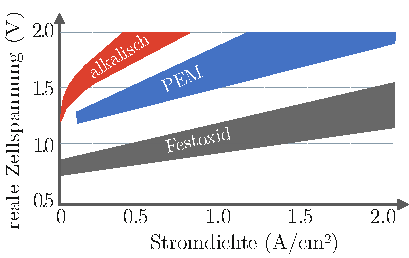
\includegraphics[scale=1]{Figures/PolarisationskurvenElektrolyseure}
		\caption{Mögliche Bereiche der Polarisationskurven der in \ref{subsec:Technologien der Wasserelektrolyse} erläuterten technischen Verfahren nach \citet{tremel_electrolysisfundamental_2018}.}
\label{fig:PolarisationskurveElektrolyseure}	
\end{figure}

Des weiteren lässt sich die Polarisationskurve auch zur Identifikation sinnvoller Betriebsbereiche nutzen:\\
Die elektrische Leistung einer Zelle ($P_{el}$) lässt sich aus der Stromdichte ($i$), der aktiven Fläche ($A_{zelle}$) und der realen Zellspannung errechnen. Das Faradaysche Gesetz liefert einen direkten Zusammenhang zwischen dem Elektronenfluss und dem Stoffmengenstrom des produzierten Wasserstoffs ($\dot{n}_{H_2O}$).
\begin{align}
	P_{el}(i) = &U_{real}(i)\cdot i A_{zelle}\\
	\dot{n}_{H_2O} = &\frac{i A_{zelle}}{zF}
	\label{gl:n_i}
\end{align}
Der Wirkungsgrad ($\eta$) einer Zelle, bezogen auf den unteren Heizwert ($H_u$) von Wasserstoff wird damit durch folgenden Ausdruck beschrieben:
\begin{align}
	\eta = \frac{H_u \cdot\dot{n}_{H_2O}}{P_{el}} = \frac{H_u}{U_{real}(i)\cdot{zF}}
\end{align}
Somit zeigt sich, dass es zur Steigerung der Effizienz erstrebenswert ist, den Elektrolyseur bei einer niedrigen Spannungen zu betreiben \citep{biaku_semiempirical_2008}. Aus Abbildung \ref{fig:PolarisationskurveElektrolyseure} wird ersichtlich, dass dies bei einer niedrigen Stromdichte der Fall ist. Allerdings bleibt zu bedenken, dass dadurch auch der Produktgas Strom verringert wird. Daher ist bei der Auslegung ein Kompromiss zwischen Wirkungsgrad und einer größeren aktive Zellfläche - und damit verbunden höheren Investitionskosten und größerem Bauraum - zu finden.\\
Weiterhin stellt die Gasreinheit der Produktströme eine untere Betriebsgrenze für die Stromdichte dar. Aufgrund der Diffusion der Produktgase zur gegenüberliegenden Elektrode kommt es zu einer Mischung von Sauerstoff und Wasserstoff. Um die Zerstörung des Systems durch Explosionen zu verhindern, geben \citet{brauns_alkaline_2020} an, dass meist bei einer Verunreinigung über 2 Volumen-\%  ein Notstopp des gesamten Elektrolyseur-Systems eingeleitet wird. Daher werden Grenzwerte für den maximalen Betriebsdruck und die minimale Stromdichte empfohlen, weil diese beiden Größen die Gasreinheit signifikant beeinflussen.\\

\subsection{Technologien der Wasserelektrolyse}
\label{subsec:Technologien der Wasserelektrolyse}
Im Folgenden werden die drei maßgeblichen Verfahren zur Wasserelektrolyse näher erläutert und verglichen.
\paragraph{Alkalischer Elektrolyseur}
\label{par:Alkalischer Elektrolyseur}
Die alkalische Elektrolyse ist eine ausgereifte Technik und der derzeitige Standard für groß dimensionierte Elektrolyseure \citep{tremel_electrolysisfundamental_2018}. Anlagen mit einer Eingangsleistung von bis zu \SI{130}{\mega\W}  sind derzeit im Betrieb und die minimale Teillast liegt nach \citet{guandalini_comparative_2016} bei ungefähr $\SI{20}{\%}$. Als Elektrolyt dient üblicherweise zwischen 25 und 30 prozentige Natron- (NaOH) oder Kalilauge (KOH) \citep{tremel_electrolysisfundamental_2018}. Die Konzentration beeinflusst dabei maßgeblich die Leitfähigkeit der Lösung. Als Ladungsträger in der Lösung fungieren Hydroxidionen. Es werden metallische Elektroden verwendet, welche zur Steigerung der Aktivität mit Edelmetallen beschichtet werden können. Folgende Reaktionen laufen an der Kathode und Anode ab:
\begin{align}
  \ce{	&{Kathode:} &2H2O + 2 e^- &-> H2 + 2OH^-\\
  		&{Anode:} &2OH^- &-> H2O + O2 + 2 e^-} 
\end{align}
Um die produzierten Gase voneinander getrennt zu halten, wird zwischen Anode und Kathode ein Diaphragma positioniert. Dies hat neben Performance- auch Sicherheitsgründe, da elementarer Wasserstoff hochentzündlich ist. Aus diesem Grund sind Elektrolyseure auch in ihrer Dynamik eingeschränkt: Bevor das System abgeschaltet werden kann, müssen die Gasleitungen mit Inertgas gefüllt werden, um die Bildung einer explosiven Wasserstoff-Sauerstoff Mischung zu verhindern. Dies hat auch einen Einfluss auf den Anlaufvorgang des Systems, da die Gasqualität durch die anfangs vorliegenden Inertgase vermindert wird. Nach \citet{milanzi_technischer_2018} kann das dynamische Verhalten von Elektrolyseuren erheblich verbessert werden, wenn sie während Standzeiten im Standby betrieben werden. \\ 
Ein weiterer Nachteil aktueller technischer Anlagen der alkalischen Elektrolyse ist, dass die maximale Stromdichte verglichen mit anderen Elektrolyseuren niedrig ausfällt (\citet{tremel_electrolysisfundamental_2018} gibt Stromdichten von $0,2-\SI{0,5}{\A\per\cm\squared}$ an).

\paragraph{Protonen Austausch Membran (PEM) Elektrolyseur}
\label{par:Protonen Austausch Membran (PEM) Elektrolyseur}
PEM-Elektrolyseure werden seit 1950 entwickelt und derzeit im $\SI{1}{\mega\W}$ Bereich vertrieben. Ein Vorteil der Technologie sind die hohen erreichbaren Stromdichten von bis zu $\SI{2}{\A\per\cm\squared}$. Zudem können PEM-Elektrolyseure sehr dynamisch betrieben werden und ein Betrieb bei bis zu 10\% minimaler Teillast ist möglich \citep{tremel_electrolysisfundamental_2018}.\\
Als Ladungsträger fungieren Protonen und als Elektrolyt dient eine in destilliertem Wasser positionierte Protonen-Austausch-Membran (\textbf{P}roton \textbf{E}xchange \textbf{M}embran).
Die Protonenleitfähigkeit der Polymer-Membran wird durch Sulfonsäure-bindende Seitengruppen, sogenannte Idomere, erreicht \citep{tjarks_pem-elektrolyse-systeme_2017}.  Für die Dicke der Membran muss dabei ein Kompromiss zwischen Langlebigkeit und Durchlässigkeit gefunden werden \citep{falcao_review_2020}. Der Säuregehalt des Elektrolyts und die damit verbundene Anforderung an die Korrosionsbeständigkeit, so wie das Erstreben hoher Reaktionsgeschwindigkeiten führt zu hohen Kosten bei den Elektrodenmaterialien: Die Kathode besteht meist aus mit Platin beschichtetem Kohlenstoff, als Anode werden häufig als Oxid vorliegendes Irdium oder Ruthenium verwendet. Folgende Reaktionen laufen an der Kathode und Anode ab:
\begin{align}
  \ce{	&{Kathode:} &2H^+ + 2e^- &-> H2\\
  		&{Anode:} &H2O  &->  1/2O2 + 2H^+ + 2 e^-}
\end{align}
  		
\paragraph{Festoxid-Elektrolyseur}
\label{par:Festoxid-Elektrolyseur}
Feststoffoxid(SO) Elektrolyseure sind seit 1980 in Entwicklung \citep{tremel_electrolysisfundamental_2018}. Sie haben  den Vorteil, dass sie bei Temperaturen von $700-\SI{1000}{\degreeCelsius}$ betrieben werden, wodurch dampfförmiges Wasser zerlegt wird, wohingegen bei alkalischen und PEM-Elektrolyseuren flüssiges Wasser vorliegt. Daraus resultiert, dass Reaktionsenthalpie und dadurch auch die reale Zellspannung niedriger ausfällt. Dieser Effekt wird dadurch verstärkt, dass bei hohen Temperaturen die ohmschen Verluste sinken, wodurch niedrigere Überspannungen entstehen \citep{tremel_electrolysisfundamental_2018}. Zudem steigt mit der Temperatur auch die Reaktionsgeschwindigkeit, weshalb keine teuren Katalysator-Materialien verwendet werden müssen \citep{yan_performance_2017}.\\
Ein Nachteil der gesteigerten Betriebstemperatur sind die höheren Ansprüche an die Temperaturbeständigkeit der Elektroden und des Elektrolyts. Als Elektrolyt wird meist Zirkoniumdioxid ($\ce{ZrO2}$) verwendet, welches zur Steigerung der Leitfähigkeit mit Yttriumoxid ($\ce{Y2O3}$) stabilisiert wird \citep{butz_decomposition_2009}.
Das Elektrolyt wird zwischen zwei porösen Elektroden (Beispielsweise eine Nickeloxid Anode und eine LSCF-Kathode \citep{schiller_high_2010}) positioniert, was den Austausch der Oxidionen ermöglicht. Es existieren SO-Elektrolyseure, welche auf dem Transport von Protonen basieren, allerdings wird aufgrund ihrer geringen Bedeutung  in dieser Arbeit nicht weiter darauf eingegangen \citep{stempien_solid_2013}. Folgende Reaktionsgleichungen liegen bei den betrachteten Festoxid-Elektrolyseuren vor:
\begin{align}
  \ce{	&{Kathode:} &H2O &-> H2 + O^2- + 2e^-\\
  		&{Anode:} &O^2- + 2 e^-  &->  1/2O2} 
\end{align}
Eine Herausforderung ist das Bereitstellen der benötigten Wärme zur Wasserdampferzeugung und zum Aufrechterhalten der Betriebstemperatur. Dazu werden verschiedene Möglichkeiten, wie beispielsweise die Kopplung mit Wärmepumpen oder Sonnenkollektoren in Betracht gezogen \citep{stempien_solid_2013}. Weiterhin bleibt ein zu lösendes Problem der Leistungsverlust und der Abbau der Elektrodenmaterialien, was die Lebensdauer der Zellen signifikant einschränkt \citep{yan_performance_2017}.\\

Abschließend sind in Tabelle \ref{tb:VglElektrolyseur} wichtige Kennwerte der drei Technologien sowie ihre Vor- und Nachteile aufgeführt.

\begin{table}[ht]
		\centering
		\caption{Vergleich der gängigen Technologien zur Wasserelektrolyse nach \citet{milanzi_technischer_2018}, \citet{tremel_electrolysisfundamental_2018} und \citet{rashid_hydrogen_2015}.}
		\begin{tabular}{l c c c}
		\toprule
		 & alkalisch & PEM & Festoxid
		\\
		\midrule
		Temperatur & $40 - \SI{90}{\degreeCelsius}$ & $20 - \SI{100}{\degreeCelsius}$ & $700-\SI{1000}{\degreeCelsius}$\\
		min. Teillast & 20\% & 10\% & 30\% \\
		max. Stromdichte & $0,2 - \SI{0,5}{\A\per\cm\squared}$ & $\SI{2}{\A\per\cm\squared}$ & $\SI{1}{\A\per\cm\squared}$\\
		max. Lastgradient & $\SI{33}{\%\per\s}$ & $\SI{100}{\%\per\s}$ & \\
		\midrule
		Vorteile & geringer Preis & Kompaktheit & Wirkungsgrad\\
		& Technologiereife & Betriebsbereich & günstiger Katalysator\\
		& Lebensdauer & Lastgradient & hoher Betriebsdruck\\
		& & Gasreinheit&\\
		\midrule
		Nachteile & geringe Gasreinheit & hohe Kosten & Technologiereife\\
		& korrosives Elektrolyt & saures Elektrolyt & Lebensdauer\\
		& geringer Betriebsdruck & lange Anfahrzeit & \\
		\bottomrule
		\end{tabular}
		\label{tb:VglElektrolyseur}
\end{table}	


\subsection{Grundlagen von Brennstoffzellen}
\label{subsec:BZ}
In Brennstoffzellen wird der Umkehrprozess der Elektrolyse betrieben. Die chemische Reaktionsenergie eines Kraftstoffes wird in elektrische Energie umgewandelt. Bei Wasserstoff betriebenen Brennstoffzellen läuft die Reaktion \ref{gl:Reaktionsgleichung} rückwärts ab, es wird aus Wasserstoff und Sauerstoff Wasser gebildet. Der Aufbau von Brennstoffzellen gleicht dem von Elektrolyseuren: Es werden zwei Elektroden, ein Elektrolyt sowie gegebenenfalls ein Diaphragma zur Gastrennung verwendet. Daher werden einige Zellen sowohl als Brennstoffzelle als auch als Elektrolyseur eingesetzt \citep{yan_performance_2017}. Ein Vorteil der Brennstoffzelle ist dabei, dass sowohl reiner Sauerstoff als auch Umgebungsluft zur Kombination mit Wasserstoff verwendet werden kann \citep{olabi_prospects_2020,jiao_challenges_2017}.\\
Die in \ref{subsec:Elektrochemische Betrachtung} genannten elektrochemischen Grundlagen lassen sich auf die Brennstoffzelle übertragen: Die reversible Zellspannung $U_{rev}$ entspricht der maximalen Ausgangsspannung der Brennstoffzelle. Weil $U_{rev} < U_{th}$ wird stets weniger elektrische Energie abgeführt, als chemische Energie zugeführt wird, es liegt also eine exotherme Reaktion vor. Da die in \ref{subsubsec:Überspannungen} beschriebenen Verlustmechanismen durch Diffusionsvorgänge und ohmsche Widerstände hervorgerufen werden, treten sie auch bei Brennstoffzellen auf \citep{chugh_experimental_2020}. Allerdings werden die Verlustterme von der reversiblen Zellspannung subtrahiert:\\
\begin{align}
	\label{gl:U_real-BZ}
	U_{real} =  U_{rev} - U_{Akt} - U_{Ohm} - U_{Diff}
\end{align}   

Wie auch bei Elektrolyseuren existieren für die Umsetzung von reinem Wasserstoff alkalische, PEM und Festoxid Brennstoffzellen \citep{lucia_overview_2014}. Auf weitere Technologien, welche Methan, Erdgas oder vergaste Kohle als Energieträger verwenden wird in dieser Arbeit nicht näher eingegangen.\\
Während die elektrochemischen Grundlagen der Brennstoffzelle bereits im 19. Jahrhundert entdeckt wurden, entwickelte die NASA   gegen Ende der 1950er die ersten alkalischen und PEM Brennstoffzellen für Raumfahrtanwendungen. Auffällig ist, dass im Gegensatz zur Elektrolyse, bei der heutzutage bei großen Anlagen alkalische Elektrolyseure der Stand der Technik sind (\ref{par:Alkalischer Elektrolyseur}), bei den Brennstoffzellen die PEM-Technologie deutlich verbreiteter ist. So gibt \citet{lucia_overview_2014} an, dass 2010  der Marktanteil der PEM-Technologie bei Brennstoffzellen bei 97\% lag. Eine mögliche Erklärung dafür ist, dass Brennstoffzellen vorwiegend bei mobilen Anwendungen eingesetzt werden - nach \citet{lucia_overview_2014} ist dies bei 95\% aller verkauften Brennstoffzellen der Fall. Die Vorteile von Brennstoffzellen sind dabei die geringen Geräusch- und Schadstoffemissionen \citep{olabi_prospects_2020}. Für mobile Anwendungen eignen sich insbesondere PEM-Brennstoffzellen, da diese bei einer höheren maximalen Stromdichte betrieben werden können als alkalische und Festoxid-Zellen. Das wiederum bringt  Vorteile im Bezug auf den benötigten Bauraum und das Gewicht mit sich.\\ 
Eine weiteres Anwendungsgebiet von Brennstoffzellen ist aufgrund des exothermen Betriebs die Kraft-Wärme-Kopplung. \citet{olabi_prospects_2020} geben an, dass Brennstoffzellen höhere Gesamt-Wirkungsgrade erreichen als andere klein-skalierte Systeme zur Kraft-Wärme-Kopplung. Dabei ist zu beachten, dass die Qualität der Abwärme insbesondere von der Betriebstemperatur der Brennstoffzelle abhängt, was nach Tabelle \ref{tb:VglBz} für den Einsatz von Festoxid-Brennstoffzellen spricht.\\ 
In Tabelle \ref{tb:VglBz} werden wichtige Kennwerte der drei Technologien sowie ihre Vor- und Nachteile angegeben.\\

\begin{table}[ht]
		\centering
		\caption{Vergleich der gängigen Technologien Wasserstoff-basierter Brennstoffzellen nach \citet{mekhilef_comparative_2012}.}
		\begin{tabular}{l c c c}
		\toprule
		 & alkalisch & PEM & Festoxid
		\\
		\midrule
		Temperatur & $90 - \SI{100}{\degreeCelsius}$ & $50 - \SI{100}{\degreeCelsius}$ & $600-\SI{1000}{\degreeCelsius}$\\
		el. Wirkungsgrad & 60\% & 53-58\% & 35-43\% \\
		ges. Wirkungsgrad & 80\% & 70-90\% & 80\%\\
		\midrule
		Vorteile & Preis & Kompaktheit & günstiger Katalysator\\
		& Technologiereife & Lebensdauer & Effizienz\\
		&  & kurze Anfahrzeit & \\
		\midrule
		Nachteile & Empfindlich bei $\ce{CO2}$ &  & Technologiereife\\
		& korrosives Elektrolyt & saures Elektrolyt & Lebensdauer\\
		& geringer Betriebsdruck & & lange Anfahrzeit\\
		\bottomrule
		\end{tabular}
		\label{tb:VglBz}
		\end{table}	
		
\subsection{Benötigte Systemkomponenten}
\label{subsec:Systemkomponenten}
Die zum Betrieb von Elektrolyseuren und Brennstoffzellen benötigt Komponenten werden in dem folgenden Abschnitt erläutert,  da sie einen wesentlichen Einfluss auf das Verhalten des Gesamtsystems haben. Abbildungen \ref{fig:ProzessElektrolyse} sowie \ref{fig:ProzessBrennstoffzelle} liefern dazu einen Überblick.

\begin{figure}[h]
	\centering
		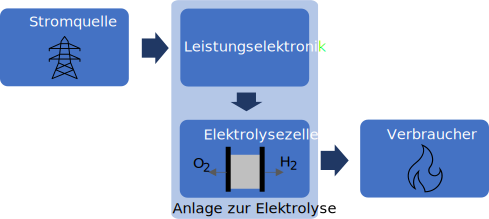
\includegraphics[scale=1]{Figures/ElektrolyseurProzessschritte}
		\caption{Übersicht der benötigten Systemkomponenten zum Betrieb eines Elektrolyseurs \citep{tjarks_pem-elektrolyse-systeme_2017}.}
\label{fig:ProzessElektrolyse}	
\end{figure}

\begin{figure}[h]
	\centering
		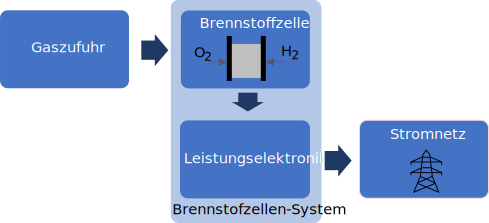
\includegraphics[scale=1]{Figures/BrennstoffzelleProzessschritte}
		\caption{Übersicht der benötigten Systemkomponenten zum Betrieb einer Brennstoffzelle.}
\label{fig:ProzessBrennstoffzelle}	
\end{figure}

Im Falle der Elektrolyse wird die Leistungselektronik benötigt, um zwei Aufgaben zu erfüllen:
Erstens die Anpassung der Versorgungsleistung auf die elektrischen Anforderungen des Elektrolyseurs und zweitens die Wandlung der Wechselspannung zu Gleichspannung \citep{tjarks_pem-elektrolyse-systeme_2017}.
Stand der Technik sind Thyristor-basierte Gleichrichter, welche sich durch geringe Verluste auszeichnen.
Als Nachteil dieser Technik ist allerdings zu nennen, dass die Schaltfrequenz an die Netzfrequenz gekoppelt ist, was die Restwelligkeit der Ausgangsgrößen erhöht.
Transistor-basierte Gleichrichter versprechen im Bereich der Restwelligkeit wesentliche Verbesserungen und durch aktuelle Entwicklungen konnten die auftretenden Schaltverluste  signifikant verringert werden \citep{tjarks_pem-elektrolyse-systeme_2017}.\\

Im Falle der Brennstoffzelle wird die Leistungselektronik benötigt, um die erzeugte Gleichspannung zu Wechselspannung zu transformieren und den elektrischen Anforderungen des Netzes anzupassen.
Nach \citet{engler_wechselrichter_nodate} haben sich im Bereich der Wechselrichter Transistor-basierte Systeme etabliert.
Häufig werden Niederfrequenz Transformatoren verwendet, welche sich durch eine hohe Zuverlässigkeit auszeichnen, allerdings Nachteile bei dem Gewicht und der Baugröße aufweisen.
Ein Entwicklungsfeld sind daher Hochfrequenztransformatoren, die ein geringeres Gewicht und einen kleineren Bauraum ermöglichen.